%%%%%%%%%%%%%%%%%%%%%%%%%%%%%%%%
%%%
%%% Research Summary
%%%
%%% Author - Steve Hurder
%%%
%%% Date Started: October 12, 2009
%%% Date Completed: November 15 , 2009
%%%%%%%%%%%%%%%%%%%%%%%%%%%%%%%% [11pt]{amsart}

\documentclass[11pt]{amsart}
% Copyright (c) 2012 Cies Breijs
%
% The MIT License
%
% Permission is hereby granted, free of charge, to any person obtaining a copy
% of this software and associated documentation files (the "Software"), to deal
% in the Software without restriction, including without limitation the rights
% to use, copy, modify, merge, publish, distribute, sublicense, and/or sell
% copies of the Software, and to permit persons to whom the Software is
% furnished to do so, subject to the following conditions:
%
% The above copyright notice and this permission notice shall be included in
% all copies or substantial portions of the Software.
%
% THE SOFTWARE IS PROVIDED "AS IS", WITHOUT WARRANTY OF ANY KIND, EXPRESS OR
% IMPLIED, INCLUDING BUT NOT LIMITED TO THE WARRANTIES OF MERCHANTABILITY,
% FITNESS FOR A PARTICULAR PURPOSE AND NONINFRINGEMENT. IN NO EVENT SHALL THE
% AUTHORS OR COPYRIGHT HOLDERS BE LIABLE FOR ANY CLAIM, DAMAGES OR OTHER
% LIABILITY, WHETHER IN AN ACTION OF CONTRACT, TORT OR OTHERWISE, ARISING FROM,
% OUT OF OR IN CONNECTION WITH THE SOFTWARE OR THE USE OR OTHER DEALINGS IN THE
% SOFTWARE.

%%% LOAD AND SETUP PACKAGES

\usepackage[margin=0.5in]{geometry} % Adjusts the margins

\usepackage{multicol} % Required for multiple columns of text

\usepackage{mdwlist} % Required to fine tune lists with a inline headings and indented content

\usepackage{relsize} % Required for the \textscale command for custom small caps text

\usepackage[pdftex]{hyperref} % Required for customizing links
\usepackage[dvipsnames]{xcolor} % Required for specifying custom colors
\definecolor{dark-blue}{rgb}{0.15,0.15,0.4} % Defines the dark blue color used for links
\hypersetup{colorlinks,linkcolor={dark-blue},citecolor={dark-blue},urlcolor={dark-blue}} % Assigns the dark blue color to all links in the template

\usepackage{tgpagella} % Use the TeX Gyre Pagella font throughout the document
\usepackage[T1]{fontenc}
\usepackage{microtype} % Slightly tweaks character and word spacings for better typography

\pagestyle{empty} % Stop page numbering

%----------------------------------------------------------------------------------------
%	DEFINE STRUCTURAL COMMANDS
%----------------------------------------------------------------------------------------

\newenvironment{indentsection} % Defines the indentsection environment which indents text in sections titles
{\begin{list}{}{\setlength{\leftmargin}{\newparindent}\setlength{\parsep}{0pt}\setlength{\parskip}{0pt}\setlength{\itemsep}{0pt}\setlength{\topsep}{0pt}}}{\end{list}}

\newcommand*\maintitle[2]{\noindent{\LARGE \textbf{#1}}\ \ \ \emph{#2}\vspace{0.3em}} % Main title (name) with date of birth or subtitle

\newcommand*\roottitle[1]{\subsection*{#1}\vspace{-0.3em}\nopagebreak[4]} % Top level sections in the template

\newcommand{\headedsection}[3]{\nopagebreak[4]\begin{indentsection}\item[]\textscale{1.1}{#1}\hfill#2#3\end{indentsection}\nopagebreak[4]} % Section title used for a new employer

\newcommand{\headedsubsection}[3]{\nopagebreak[4]\begin{indentsection}\item[]\textbf{#1}\hfill\emph{#2}#3\end{indentsection}\nopagebreak[4]} % Section title used for a new position

\newcommand{\bodytext}[1]{\nopagebreak[4]\begin{indentsection}\item[]#1\end{indentsection}\pagebreak[2]} % Body text (indented)

\newcommand{\inlineheadsection}[2]{\begin{basedescript}{\setlength{\leftmargin}{\doubleparindent}}\item[\hspace{\newparindent}\textbf{#1}]#2\end{basedescript}\vspace{-1.7em}} % Section title where body text starts immediately after the title

\newcommand*\acr[1]{\textscale{.85}{#1}} % Custom acronyms command

\newcommand*\bull{\ \ \raisebox{-0.365em}[-1em][-1em]{\textscale{4}{$\cdot$}} \ } % Custom bullet point for separating content

\newlength{\newparindent} % It seems not to work when simply using \parindent...
\addtolength{\newparindent}{\parindent}

\newlength{\doubleparindent} % A double \parindent...
\addtolength{\doubleparindent}{\parindent}

\newcommand{\breakvspace}[1]{\pagebreak[2]\vspace{#1}\pagebreak[2]} % A custom vspace command with custom before and after spacing lengths
\newcommand{\nobreakvspace}[1]{\nopagebreak[4]\vspace{#1}\nopagebreak[4]} % A custom vspace command with custom before and after spacing lengths that do not break the page

\newcommand{\spacedhrule}[2]{\breakvspace{#1}\hrule\nobreakvspace{#2}} % Defines a horizontal line with some vertical space before and after it


\newcommand{\grant}[7]{

\headedsubsection{#1}{#2--#3 (#4)} { % title, start date, end date, source
	\inlineheadsection{Investigators:}{#5}
	\vspace{1.2em}
	\inlineheadsection{Award:}{\$#6 (Share: \$#7)}
	\vspace{1.2em}
}
}

\newcommand{\colabgrant}[8]{

\headedsubsection{#1}{#2--#3 (#4)} { % title, start date, end date, source
	\inlineheadsection{Investigators:}{#5}
	\vspace{1.2em}
	\inlineheadsection{Award:}{\$#6 (Share: \$#7)}
	\vspace{1.2em}
	\inlineheadsection{Collaboration:}{#8}
	\vspace{1.2em}
}
}


\newif\ifumd\umdtrue
\usepackage{graphicx}
\usepackage{amssymb}
\usepackage{mfirstuc}
\usepackage{colortbl}
\usepackage{epstopdf}
\usepackage{multicol}
\usepackage{url}

\newcommand{\abr}[1]{\textsc{#1}}
\newcommand{\newcite}[2]{\capitalisewords{#1} et al.~\cite{#1-#2}}



\newcommand{\student}[1]{\vspace{.5cm}\fbox{\parbox{0.95\linewidth}{{\small
        #1}}}\vspace{.5cm}}
\providecommand{\blue}[1]{{\color{blue}{#1}}}
\providecommand{\red}[1]{{\color{red}{#1}}}
\providecommand{\green}[1]{{\color{green}{#1}}}

\begin{document}


 \title{Personal Statement: Evaluating and Enabling Human--AI Collaboration}

 \author{Jordan Boyd-Graber, University of Maryland}
%\institute{University of Colorado, Boulder CO 80309, USA}


%\date{May 2023}

\maketitle

Artificial intelligence\footnote{I take a broad interpretation of
\abr{ai}; some of my examples might be better characterized machine
learning.  But rather than distracting boundary policing, I will embrace
the general term but will be specific in describing particular tools/models.}
(\abr{ai}) is ubiquitous: detecting spam e-mails, flagging fraudulent
purchases, and providing the next movie in a Netflix binge.
%
But they do not exist in a vacuum: as
Shneiderman~\cite{shneiderman-21} argues, \abr{ai} must exist
alongside humans.
%
My goal is to create metrics to measure whether \abr{ai} methods make
sense to users, help users craft examples to advance \abr{ai}, and
applying \abr{ai} to illuminate complex social
science applications.

\section{Evaluating Interpretability}

My journey with evaluating interpretability began over ten years ago
with topic models.
%
Topic models are sold as a tool for understanding large data
collections: lawyers scouring Nordstream e-mails for a smoking gun,
journalists making sense of Wikileaks, or humanists characterizing the
oeuvre of Lope de Vega.
%
But topic models' proponents never asked what those lawyers,
journalists, or humanists needed.
%
Instead, they optimized \emph{held-out likelihood}.

When my colleagues
and I developed the \emph{interpretability} measure to assess whether topic
models' users understood their outputs, interpretability and
held-out likelihood were negatively correlated~\cite{chang-09b}!
%
% The topic modeling community (including me) had fetishized complexity
% at the expense of usability\dots and topic modeling is not alone.

\begin{center}
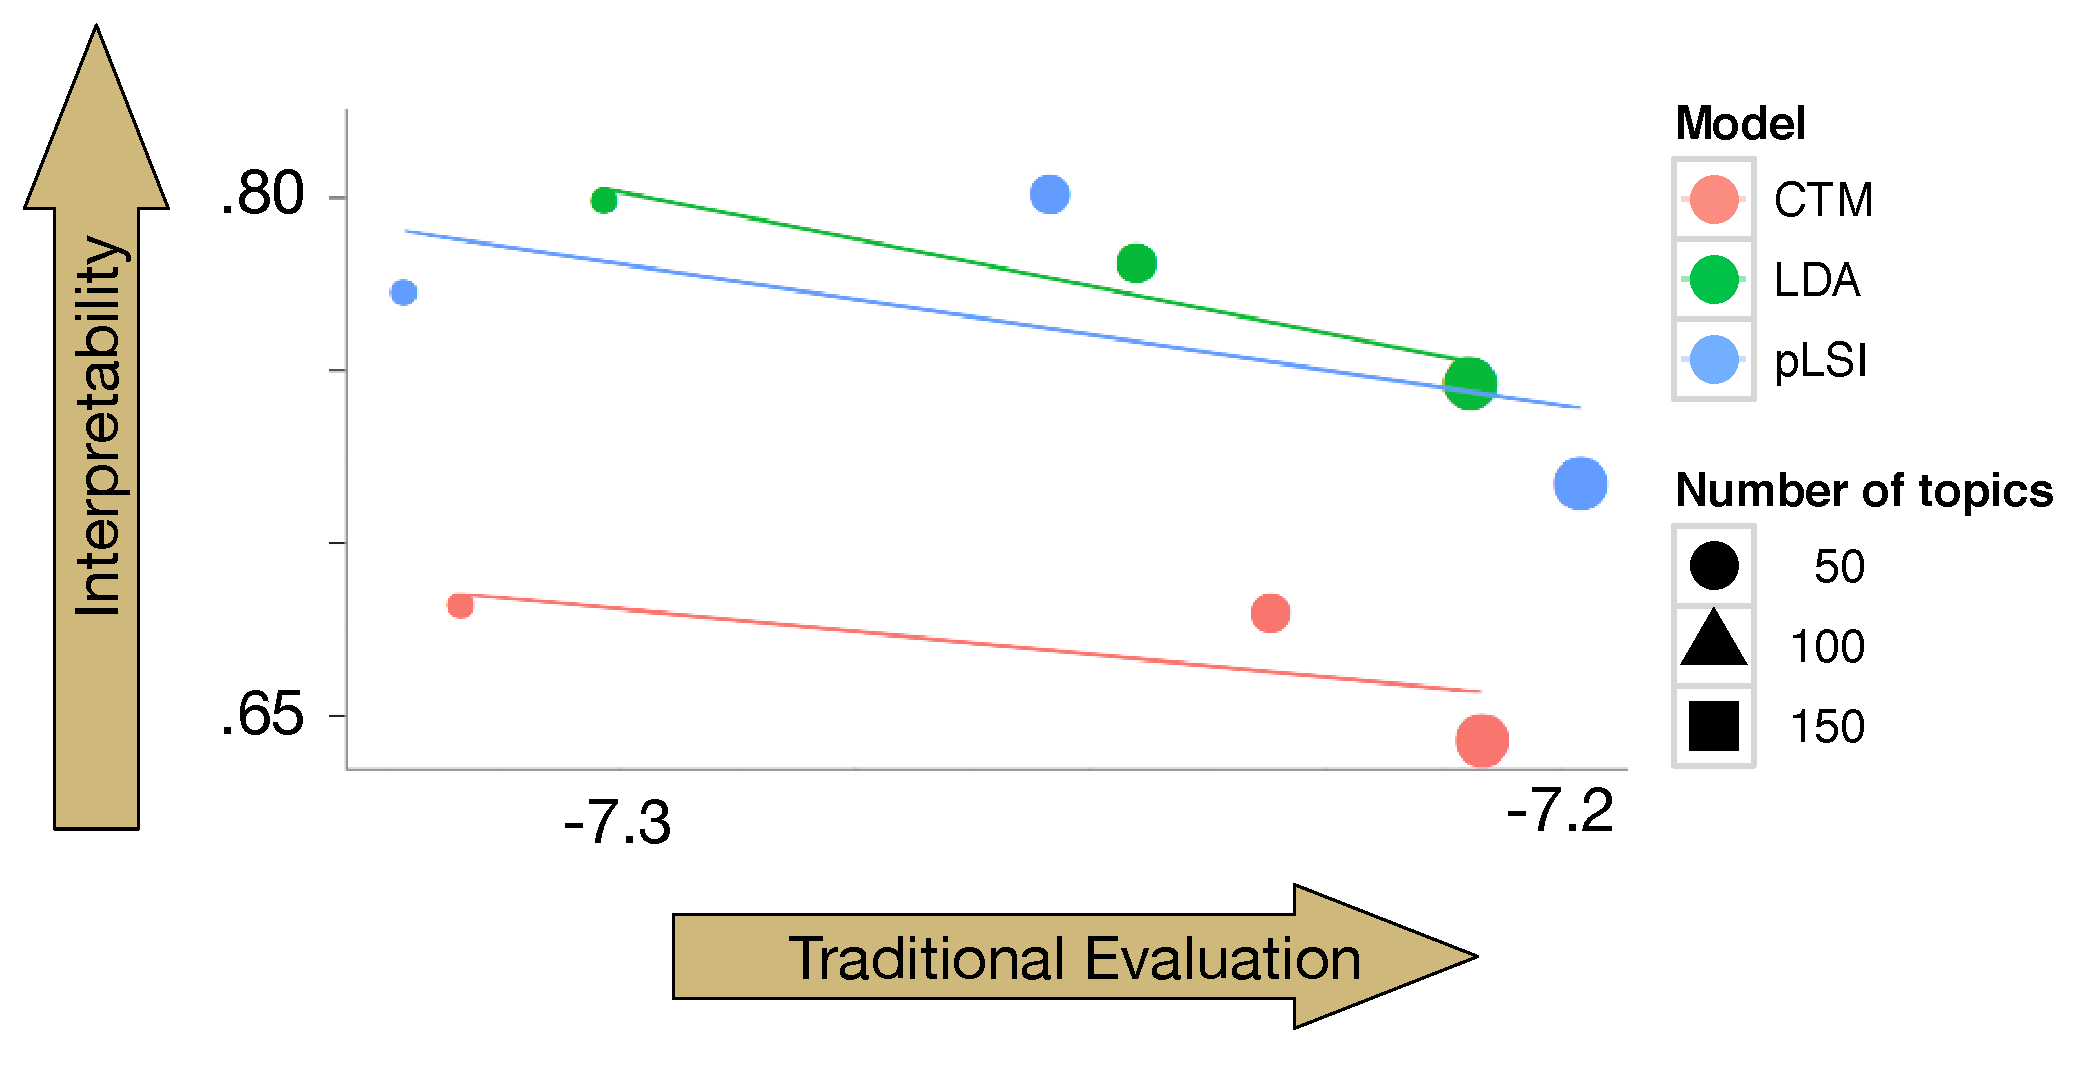
\includegraphics[width=.5\linewidth]{images/prec_ll_4}
\end{center}

Since this humbling discovery, I've built topic models that are a
collaboration between humans and computers~\cite{hu-14:itm}, an
improvement over the ``take it or leave it'' philosophy of most
machine learning algorithms.

Focusing on collaboration also requires algorithms that are low
latency (not just high throughput), extending
geometric interpretations of Arora et
al.~\cite{arora-12} to multi-anchor topics~\cite{lund-17} and
multi-lingual topics~\cite{Yuan-18}, models that can handle millions of documents in seconds.
%
% We also developed better understanding of the projections of
% multilingual representations via graph theory~\cite{Fujinuma-19} and
% the convergence of alternating projections~\cite{Zhang-19}.

After our ``reading tea leaves'' evaluation, it's
heartening that \newcite{lau}{14} and their ``machine reading tea
leaves'' (which correlate with our human measures) became a standard
topic model evaluation: in a survey of forty recent topic modeling
papers, {\bf all but four} use a form of their coherence evaluation.
%
However, as we argue in \newcite{hoyle}{21}, you cannot just use this
evaluation forever and forget about humans.
%
In that same survey, {\bf none} of those papers do a human evaluation.
%
As topic models evolve (e.g., incorporating
neural components), you need to validate that these automatic metrics
still correlate with whether it is useful for a human--computer
collaboration.

\section{Teaming as an Evaluation}

Within the \abr{hci}, we have argued for 
what should go into human--computer collaborations: computers that incorporate
users' suggestions~\cite{kumar-19}; explanations with
accountability~\cite{smith-20}; and stable
explanations~\cite{smith-20:adherence}.

In addition to these human-centered understanding of users' needs and
desires, we've developed machine learning approaches to measure how
well users complete a task.
%
For example, for a question answering task, we measured how much the
accuracy of the human--computer \emph{team} increases with different
explanations and found that explanations help all users but that
novices are easily overwhelmed~\cite{feng-19}.
%
In follow-on work, we learned how to explicitly optimize explanations
for individual users~\cite{feng-22}.


\section{Connecting with Social Science: Pedagogy, Framing, and Deception}

The reverse of cooperation is human competition; it also has much to
teach computers.
%
I've increasingly looked at language-based games whose clear goals and
intrinsic fun speed research progress.
%
For example, in the board game \emph{Diplomacy}, users
chat with each other while marshaling armies for world conquest. Alliances are
fluid: friends are betrayed and enemies embraced as the game develops.
%
However,
users' conversations let us predict when friendships break.

Thus, we argued that Diplomacy would be an exciting testbed for
natural language processing, and our 2015 paper is---to the best of
our knowledge---the first \abr{nlp} research on Diplomacy.
%
Before a betrayal, betrayers write ostensibly friendly messages and become more polite, stop talking about the future, and change how \emph{much} they write~\cite{niculae-15}.
%
In follow-on work, we developed a dataset that predict both when users
lie to each other and when recipients of lies detect
deception~\cite{Peskov-20}.
%
We are continuing to look into these questions with researchers from
across the nation in a new \abr{darpa} program: \abr{shade}, which
focuses on Diplomacy as a testbed for understanding deception.

Recently, the use of \abr{nlp} methods in the game of Diplomacy has
been the subject of highly-publicized papers by DeepMind in Nature
Communications~\cite{kramar-22} and Meta in Science~\cite{bakhtin-22}.
% %
% The Meta paper, like our 2020 paper, used a classifier to detect
% deceptive statements.
% %
% The DeepMind paper built a game theoretic understanding of when
% betrayal should happen, building on our descriptive investigation of
% deception in human games.

% A game with higher stakes is politics. However, just like Diplomacy,
% the words that people use reveal their underlying goals; computational
% methods can help expose the ``moves'' political players can use. With
% collaborators in political science, we've built models that: show when
% politicians in debates strategically change the topic to influence
% others~\cite{nguyen-12,Nguyen-14b}; frame topics to reflect political
% leanings~\cite{nguyen-13:shlda}; use subtle linguistic phrasing to
% express their political leaning~\cite{iyyer-14a}; or create political
% subgroups with larger political
% movements~\cite{Nguyen:Boyd-Graber:Resnik:Miler-2015}.

% Because political discourse is built on a common set of commonly
% accepted facts, we have focused on developing fact checking: datasets
% for general knowledge fact checking~\cite{eisenschlos-21} and climate
% change fact checking~\cite{Diggelmann-20}.
% %
% However, because fact checking is part of an information arms race, we
% need to build these examples as part of a human-in-the-loop
% adversarial process, which I'm exploring in an ongoing collaboration
% with journalism professor Naeemul Hassan that extends my question
% answering work, which I talk about next.

\section{Human-in-the-Loop Adversarial Examples}

One of the most fun aspects of my research has been building
trivia-playing robots~\cite{boyd-graber-12,iyyer-14b,iyyer-15}; beyond research papers, our system has faced off against former Jeopardy
champions in front of hundreds high school
students\footnote{\url{https://www.youtube.com/watch?v=LqsUaprYMOw}}
and against researchers at NeurIPS 2015 (which won the best
demonstration award).
%
But after defeating some of the smartest trivia players, did I
actually believe that our system was better at question answering?
%
No!

Adversarial examples first came out of the vision community: add a
small epsilon to an example and suddenly a object detector calls a
turtle a gun~\cite{athalye-18}.\footnote{Point of personal pride: I
mentored Kevin on another research project~\cite{he-16}, but
I myself had nothing to do with this later adversarial work.}
%
While others have attempted to create adversarial examples for
language using paraphrasing, it's hard to know if the changes are
perceptually negligible (``who wrote the invisible man''---a question with the answer H.G. Wells---is
fundamentally different from ``who wrote the man you can't see''---an ill-formed questions---as is
``who wrote the book invisible man''---a question with the answer Ralph Ellison) and
it's hard to ``add epsilon'' to a discrete word.

Consistent with the theme of my research, my \abr{nsf career} grant
added a \emph{human in the loop} to generate novel adversarial
language examples that can provide new training examples to make
\abr{ai} more robust and to expose what \abr{ai} cannot (yet) do.
%
With Eric Wallace, an undergraduate student, we built a system that
could help an expert trivia question writer to stump a computer: as
the author writes the question, it shows the author what the system is
thinking~\cite{wallace-18}.
%
And it worked, even generalizing across models~\cite{wallace-19} (an
example written with an \abr{ir} model still stumps a neural model); we saw similar effects with fact checking~\cite{eisenschlos-21}.
%
After we introduced human-in-the-loop adversarial example generation,
Meta/Facebook adopted this framework with gusto~\cite{bartolo-20} in
their Dynabench framework, the Dynamic Adversarial Data Collection
workshop and call for proposals (which I'm grateful is funding our
continuing research in this area).

\section{But wait, there's more!}

Many of our best-cited papers are ``traditional'' papers that do
better on some task:
%
\begin{itemize*}
\item We developed deep averaging networks~\cite[\abr{dan}]{iyyer-15}, a simple model still used in the 
transformer age~\cite{ye-22}.

\item In question answering, we proposed new evaluation mechanisms
  for knowing if an answer is correct~\cite{si-21} and improved
  information retrieval to answer complicated
  questions~\cite{elgohary-19,zhao-21,shi-20}.
  
\item We also introduced reinforcement learning to \emph{simultaneous
machine interpretation}~\cite{Grissom:He:Boyd-Graber:Morgan-2014}, a
  language-based task that requires significant human intuition,
  insight, and---for those who want to become
  interpreters---training.\footnote{This framework---using
  reinforcement learning to capture human strategies---was featured in
  Liang Huang's \abr{acl} keynote.} We learned tricks from
  professional human interpreters---passivizing sentences and guessing
  the verb---to translate sentences sooner~\cite{He-15}, letting
  speakers and algorithms cooperate together and enabling more natural
  cross-cultural communication.  We also use reinforcement
  learning to learn machine translation feedback from noisy
  supervision such as star ratings on a webpage~\cite{nguyen-17}.
\end{itemize*}

This work doesn't \emph{yet} fit nicely into the human--computer
collaboration narrative, but these more complex tasks are part of my
broader vision for where my research will go: state-of-the-art models
built to support human decisions, not replace them.  And that requires
the low-latency models built to react to input ``like a human''
described above.

\section{Future Work}

I hope that I've convinced you that to get more effective \abr{ai}, we
need to measure how well it works (and plays) \emph{with} humans.
%
This is a problem that requires solutions in the form of new data, algorithms, and evalutions, and I
hope to advance in all three areas.

{\bf Data.}
%
In new a \abr{nih} grant, we're working with answering
questions in complicated, code-switched environments with
less educated users navigating \abr{us} healthcare.
%
These linguistically, acoustically, and socio-economically diverse
samples will provide more realistic data, replete with false presuppositions, ambiguity, and
shifting information needs; we are building pragmatically grounded tools to engage with users, correct wrong assumptions, and answer their questions.
%
We are also working with \abr{nist} to develop data that 
reflect \emph{cultural} contexts: detecting when questions
are answered differently in Ghana than in the \abr{us} or topics that
only people in Bhutan care about (and thus absent in
\abr{us}-centric datasets).

{\bf Algorithms.} In research recently funded by Meta, we are \emph{learning} how to help users best
engineer adversarial examples, a natural extension of our work using
bandit algorithms to improve explanations.

However, those algorithms are for \emph{supervised} tasks where there
is a known answer.
%
For \emph{unsupervised} tasks like understanding the themes in a
document collection, we need algorithms
that are not just transparent but that are \emph{low latency}: the primary
goal is exploration of the dataset, and the user needs to be able to
quickly provide feedback to the algorithm.
%
While eventually we will need to connect to expensive, difficult to
compute neural models, many user updates can be approximated by fast
spectral or probabilistic algorithms.

{\bf Evaluation.}
%
Where computers have strengths that go beyond what a human can do, we
need to know if it would be wise to build evaluations that can we
will build interactive systems that help users come to a correct
answer through a process they trust, measure that process, and
optimize to encourage this cooperation.
%
This requires basic engineering---ensuring all of the components of
a system are efficient and low latency---and user modeling, as we
cannot assume that every user will have the same knowledge and
capabilities.
%
% The next step requires careful vetting in diverse domains to validate
% that users' skills and knowledge are actually augmented by the help of
% the computer.
%
% We aim to focus on multiple areas: question answering in a single
% language~\cite{He-22}, question answering across
% languages~\cite{han-22}, and the strategic game of Diplomacy.

But interactions with individual people are not how \abr{ai} will be a
part of 21\textsuperscript{st} society: it will be interactions with
\emph{populations}.
%
Thus, we need to have models and systems that capture population-level
interactions.
%
Helping detect misinformation online, working collaboratively with
authors to craft effective counter-measures, and to propagate that
within a social network.
%
This builds on our fake news systems and our deception detection work,
but will also require deeper collaboration with social scientists and
journalists to develop the interfaces and the models to build
human--computer \abr{ai} that informs and helps society as a whole.

\section{Teaching}

I have taught courses on natural language processing at the graduate and undergraduate level, a graduate seminar on question answering, a graduate seminar on Bayesian nonparametrics, a graduate course on distributed computation, graduate machine learning, an undergraduate practical course on deep learning frameworks, an undergraduate introduction to data science, and basic computer literacy.\footnote{A full \href{http://users.umiacs.umd.edu/~jbg/static/courses.html}{list of the courses}, the most recent with lectures.}

{\bf Flipped Classrooms.}
%
In 2012, I began teaching with flipped classrooms: you
record the lectures, students watch them before class, and then you
use the normal class time to answer questions, work through exercises,
or to talk about tricky issues on homeworks.
%
Following the
suggestions of \newcite{Zappe}{09}, I keep my videos short (around 30
minutes total, edited for concision and broken into 5--15 minute
chunks).

For example, when I talk about topic models, I have videos where I:
  \begin{enumerate}
  \item \href{https://youtu.be/qvr5J9m7Gmw}{discuss with an interlocutor why
    topic modeling is important}
  \item \href{https://www.youtube.com/watch?v=fCmIceNqVog}{introduce what
    topic modeling is;}
  \item \href{https://youtu.be/-tKmyHoVZ-g}{walk through Gibbs sampling to fit
  a topic model from text data;}
  \item \href{https://youtu.be/-tKmyHoVZ-g}{discuss variational inference in
    general; and}
  \item \href{https://youtu.be/smfWKhDcaoA}{then walk through the derivation
    of variational inference for topic models.}
  \end{enumerate}
%
The technical quality of the videos have
improved considerably over the years: I've moved from just a screen
capture to a multiple camera setup with green screen.

Then in class, I answer any questions students have and then we go
through an exercise.
%
For instance, we walk through Gibbs sampling
works for a toy example.
%
Students calculate---by hand---the sampling
equation and go through the process to get the answer.

% A lot of teachers do not like the flipped classroom, and I can
% understand why.
%
% First, it's a lot of work, and it requires planning.
% When I co-taught a flipped classroom with an uninitiated professor, he
% ended up cursing my name for convincing him to take part.

There's research to suggest that the flipped classroom can help
students engage and retain information~\cite{Zuber-16}, but that's not
the real reason that I do it.
%
I do it because it helps me get to know the students better.  Computer
science is the biggest major at Maryland (over three thousand undergrads), and
\abr{ai}-adjacent fields are even more popular within that major, so my
classes are getting pretty darn big.
%
If I didn't do a flipped
classroom, I would know so many fewer students.
%
It has also helped me get to know the community; many students have come up to me at conferences to tell me that my videos helped them learn concepts; my videos have over a million views on YouTube and over ten thousand subscribers.

{\bf Projects.}
%
I want to make sure that my students can actually use their skills
once they're done with the class.  Thus, I typically end courses with
a project.  It reinforces key concepts from the course, connects those
concepts to the rest of their curriculum and research, and often
serves as a launching point to things that are useful in the real
world.  For undergraduate classes, this is more directed: in one class
they build trivia-playing robots to take on former \textit{Jeopardy!} Champions
or Victoria Groce from the American version of \textit{The
  Chase}.\footnote{\href{https://www.youtube.com/watch?v=dyaR7zT_KKg}{https://www.youtube.com/watch?v=dyaR7zT\_KKg}}

{\bf Mentoring.}
%
I'm proud of the successes of my diverse former students.
%
Seven of my former director or co-advisees (undergrad and graduate) have gone on to tenure track positions.

\section{Service}

{\bf CLIP Director.}
At the University of Maryland, I served as the director of the
Computational Linguistics and Information Processing (\abr{clip}) Lab
2018--2022 (with a pause in the middle while I was on sabbatical in
Z\"urich).
%
This required advocating for resources for the lab---money to host visitors, space to seat students, and time from technical staff to support our computational resources, transferring our storage systems to modern support and pivoting to \abr{gpu}-focused computation---and navigating the return to campus after the pandemic.

{\bf Professional Service.}
%
In 2022, after
\href{https://www.youtube.com/watch?v=3gSgNXGxzQU}{complaining about
  how hybrid conferences} created a ``separate but equal'' status for
virtual attendees, I was invited to be \abr{emnlp}'s first virtual
poster chair.
%
Our goal was use technology and prioritizing cross-modal interaction
to make sure that those unable to be in Abu Dhabi---either because of
visa status, health, or family obligations---are still able to
interact and be visible.

After accepting this position, I was asked to serve as a program chair for the
2023 meeting of the Association for Computational Linguistics, the top venue
for natural language processing research.
%
Our goal is to further bridge the divide between the online and in-person
participants: improving the online experience, focusing on interactions, and
lowering the costs for online participants.

% TODO: Corona, virtual poster session chair

% TODO: CLIP Director

{\bf Creating a New Undergraduate Curriculum.}
%
From 2011--2013, I chaired \abr{umd}'s Information Science
undergraduate education committee. During this time, we developed a
new undergraduate degree program to complement the university's
existing strengths (and exploding enrollments) in computer science. I
developed the initial proposal, articulation agreements with local
community colleges, planned course offerings, and shepherded the
proposal through college, provost, and State of Maryland Higher
Education Commission review.
%
Susan Winter and Vedat Diker (along with many others) took over the actual
implementation of the program, which became the university's fastest growing
major (up to about a thousand majors in less than five years).


{\bf Outreach to Undergraduates and High Schools.}
% Mentoring the academic quiz team
My research is---in part---about human vs. computer question answering
competitions, so it's only natural that I also support our
undergraduate students who compete against other schools in academic
competitions by answering questions.

At the University of Colorado, I built an organization
from the ground up: the University of Colorado had previously not
competed in these events.
%
I organized three local high school tournaments to raise funds for 
students to travel to national competitions, which
they did for the first time in 2016 (after winning their region).

At Maryland, I advise an existing academic team that
consistently is in the top ten nationally.

\noindent\rule{4cm}{0.4pt}


    \parbox{\linewidth}{I have written this document and certify that this
  personal statement is a current and accurate statement of my
  professional record to the best of my
  knowledge \flushright  
\includegraphics[width=.2\linewidth]{resume_src/signature} \\
  \flushright  (\today{})}

\clearpage

\begin{multicols}{2}
  \footnotesize

\bibliographystyle{plain}
\bibliography{resume_src/journal-abbrv,resume_src/jbg}
\end{multicols}

\end{document}
